


%Tamaño y tipo de documento que queremos escribir.
\documentclass[letterpaper, 12pt,double,graphicx,caption,rotating]{book}

%Paquetes para el idioma, las tildes, etc.
\usepackage{longtable}
\usepackage[activeacute,spanish]{babel}
\usepackage[letterpaper,left=3cm,right=2.0cm]{geometry}
\usepackage[utf8]{inputenc}
\usepackage{multirow}
\usepackage{multicol}
\usepackage{parskip}
\renewcommand{\baselinestretch}{1.5}

\parskip  0.5cm
%Abrimos el bloque para escribir el documento.
\begin{document}
\begin{titlepage}
\newpage
\begin{center}


UNIVERSIDAD MAYOR DE SAN SIMÓN\\
FACULTAD DE CIENCIAS Y TECNOLOGÍA\\
CARRERA: INGENIERÍA DE SISTEMAS\\[3cm]
 {\Large Sistema Web microblog para notificación de acciones aplicadas en repositorios locales de desarrollo de proyectos de software versionados con GIT.}\\[2cm]
 {\Large Proyecto de Grado, Presentado Para Optar al Diploma Académico de Licenciatura de Ingeniería de Sistemas}\\[2cm]

 {\Large Presentado por: Gary Inturias Rojas}\\[1cm]
 {\Large Tutor: Lic. Boris Marcelo Calancha Navia }\\[2cm]
 COCHABAMBA - BOLIVIA\\
 Agosto, 2009
\end{center}
\newpage
\vfill\par\noindent
\begin{flushright}
    {\Large \textbf{Dedicatoria}}\\[1cm]
    A mis padres y hermanos por\\ brindarme su apoyo incondicional. \\
\end{flushright}
\newpage


\begin{center}
{\Large \textbf{Agradecimientos}}\\[2cm]
{\leftskip=8cm
A mis padres Juan Carlos Inturias y Celida Rojas por el apoyo incondicional que me dieron a lo largo de mi vida.\\
A mis hermanos Sonia y Ruddy por el apoyo que me dieron.\\
A la Universidad\\
Al Lic. Boris M. Calancha por sus conocimientos impartidos y las sugerencias realizadas a lo largo de mi enseñanza universitaria y el apoyo en la realización de este proyecto de grado.\\
A todas las personas que de algún modo sus criticas y sus enseñanza me ayudaron para poder enfrentar los retos de la vida.\\[3cm]
\par}
\textbf{\textit{¡Muchas Gracias!}}



\end{center}

\newpage
\begin{center}
 {\Large FICHA RESUMEN}\\
\end{center}\noindent
\baselinestretch{2.0} 
El desarrollo de proyecto de software en la actualidad se encuentra a cargo de un equipo de desarrolladores, como así también los administradores del proyecto.
La comunicación entre los integrantes es esencial para el cumplimiento de los objetivos a alcanzar, para la coordinación eficaz del equipo de trabajo y la determinación de tiempos para las respectivas tareas designadas.
La dificultad de tratar con cada uno de los integrantes de forma personal aumenta según el numero que estos integran y aun mas si realizan sus trabajos a distancia, esto causa mala comprensión de las tareas a cumplir dentro del desarrollo de software. Provocando perdidas de tiempo que en el transcurso son esenciales para la culminación del proyecto.
La mayoría de sistemas de control de versiones no se encuentran integrados a un sistema microblog, el cual facilitaría las notificaciones de las acciones que efectúan en tiempo real a los ficheros de los repositorios de trabajo. Así provocando una de-sincronización causando conflictos a la hora de realizar actualizaciones en los repositorios.
GIT no es una excepción a estos posibles problemas, debido a que cada integrante del grupo de desarrollo obtiene una copia idéntica del repositorio, es una de las cualidades de los sistemas de control de versiones distribuidas.
\tableofcontents
\end{titlepage}

%Generamos un indice de los contenidos

%\documentclass[12pt]{article}
%\usepackage[latin1]{inputenc}
%\usepackage[spanish]{babel}
%\usepackage{latexsym}
%\usepackage{amssymb}
%\usepackage{amsmath}

%\setlength{\textwidth}{15cm}

%\newtheorem{ejem}{Ejemplo}
%\newtheorem{teor}{Teorema}
%\begin{document}
\chapter{PRESENTACION}
\section{INTRODUCCION}
La dependencia causada por los sistemas informáticos en casi todas las actividades realizadas en los paises, como ser la fabricación industrial, sistemas financieros, productos eléctricos, entre otros.
Hacen que estos sistemas informáticos sean construidos a traves de la ingenieria de software que comprenden de un conjunto de tecnicas y herramientas que estan en gran crecimiento debido a las exigencias , sin embargo mientras mas crezca nuestra capacidad de producir software, tambien lo hará la complejidad de los sistemas de software solicitados.
Es asi como surgen diferentes herramientas para brindar apoyo dentro de las etapas de la ingeniera de software segun cada metódología desempeñada. Una de las etapas que es imprescindible dentro de todas estas metodologías se encuentra el desarrollo de software en el cual encontramos a una herramienta si bien no es obligatoria, resulta de gran ayuda e imprescindible para la mayoria de las empresas y personas que se dedican a la elaboración de sistemas, hablamos de los sistemas de control de versiones que nos ayudan a la administracion de las distintas versiones de cada producto desarrollado.
Encontramos una gran diversidad de sistemas de control de versiones, pero en este caso hacemos incapíe a uno de los mas populares como ser GIT, un sistema no tan conocido como su adversario SubVersion, pero que denota caracteristicas ventajosas como ser la velocidad, reduccion de tamaño,entre otras. es asi como surge la idea de la aportacion de una herramienta de apoyo para el desarrollo de software, como ser la comunicacion de anuncios en tiempo real escritos por los integrantes del equipo de desarrollo como asi tambien las acciones commit realizadas en cada uno de los repositorios locales que disponen, Publicadas a traves de un sistema microblog, pero ¿porque un microblog?. las actividades realizadas por cada integrante y las acciones en los repositorios son muy dinamicas por lo tanto sirven de gran ayuda el conocimiento del estado de cada uno de ellos, y lo hacemos mediando anuncios no muy largos publicados en el sistema, a traves de forma automatica gracias a la ayuda de algunos ganchos que nos brinda el sistema de control de versiones GIT y tambien a traves del interprete de ordenes del sistema operativo, de esta manera se realizan las publicaciones de una manera menos prejuiciosa para el desarrollar, evitando perdidas de tiempo.
\section{PLANTEAMIENTO DEL PROBLEMA}
El desarrollo de proyecto de software en la actualidad se encuentra a cargo de un equipo de desarrolladores, como así también los administradores del proyecto.

La comunicación entre los integrantes es esencial para el cumplimiento de los objetivos a alcanzar, para la coordinación eficaz del equipo de trabajo y la determinación de tiempos para las respectivas tareas designadas.

La dificultad de tratar con cada uno de los integrantes de forma personal aumenta según el numero que estos integran y aun mas si realizan sus trabajos a distancia, esto causa mala comprensión de las tareas a cumplir dentro del desarrollo de software. Provocando perdidas de tiempo que en el transcurso son esenciales para la culminación del proyecto.

La mayoría de sistemas de control de versiones no se encuentran integrados a un sistema microblog, el cual facilitaría las notificaciones de las acciones que efectúan en tiempo real a los ficheros de los repositorios de trabajo. Así provocando una de-sincronización causando conflictos a la hora de realizar actualizaciones en los repositorios.

GIT no es una excepción a estos posibles problemas, debido a que cada integrante del grupo de desarrollo obtiene una copia idéntica del repositorio, es una de las cualidades de los sistemas de control de versiones distribuidas.
\section{OBJETIVOS}
\subsection{OBJETIVO GENERAL}
Desarrollar un sistema Web microblog\footnote{Microblog es un servicio que permite a sus usuarios enviar y publicar mensajes breves.
} para notificación de acciones aplicadas en repositorios locales de desarrollo de proyectos de software versionados con GIT\footnote{GIT software de sistema de control de versiones distribuido.
}.

\subsection{OBJETIVOS ESPECIFICOS}
\begin{itemize}
\item Elegir herramientas que aporten al desarrollo del sistema
\item Analizar herramientas que faciliten la integración del sistema de control 	de versiones GIT con aplicaciones Web.
\item Realizar un asistente de configuración, para la comunicación de 	repositorios con el sistema Web(lado cliente).
\item Desarrollar el sistema web microblog, que permita registrar las acciones realizadas(commit) por los desarrolladores en los repositorios locales(lado servidor).
\end{itemize}

\section{JUSTIFICACION}
El sistema web que se desea desarrollar ayudara  a los integrantes del grupo de trabajo encargados en la realización del proyecto, facilitando hacer un seguimiento de las tareas a realizar, el reporte de avances que se realizan durante el transcurso del día, así también poder compartir información y reportar errores entre el grupo.
Los proyectos gestionados con el sistema de control de versiones GIT se podrán integrar con el sistema web microblog, debido a que se hará uso de algunos ganchos(hooks) que enlazarán con el sistema y así poder notificar a los integrantes del grupo de desarrollo en tiempo real sobre las acciones(commit) realizadas en cada uno de sus repositorios locales.
\section{METODOLOGIA}
SCRUM es una metodología ágiles, toma en cuenta la situación cambiante de los requisitos del cliente, así también minimiza la necesidad de la documentación.
Organizando el desarrollo de software de un manera evolutiva en los denominados sprints(periodos que duran de 15 a 30 días).


%\end{document}

%\documentclass[12pt]{article}
%\usepackage[latin1]{inputenc}
%\usepackage[spanish]{babel}
%\usepackage{latexsym}
%\usepackage{amssymb}
%\usepackage{amsmath}

%\setlength{\textwidth}{15cm}

%\newtheorem{ejem}{Ejemplo}
%\newtheorem{teor}{Teorema}
%\begin{document}
\chapter{DESARROLLO DEL PROYECTO}
El desarrollo del proyecto esta enfocado en dos ambientes, uno en el lado cliente, que se desarrollaron scripts para poder permitir la comunicación de los repositorios en GIT.
El otro lado el desarrollo del servidor para la elaboración del sistema web, que mantendrá informado a los desarrolladores
\section{METODOLOGÍA DE DESARROLLO}
El desarrollo del proyecto 'Desarrollar un sistema Web microblog para notificación de acciones aplicadas en repositorios locales de desarrollo de proyectos de software versionados con GIT', Esta basado en la metodología de desarrollo SCRUM.

\begin{figure}[htb]
\centering
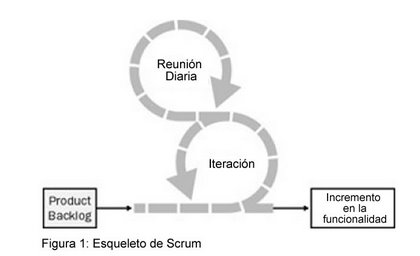
\includegraphics[width=0.7\textwidth]{imagenes/image-0.png}%ext=pdf,jpg,png
\caption{ciclos de la metodología}
\label{contexto:figura}
\end{figure}

\subsection{SCRUM}
Scrum es un proceso en el que se aplican de manera regular un conjunto de mejores prácticas para trabajar en equipo y obtener el mejor resultado posible de un proyecto. Estas prácticas se apoyan unas a otras y su selección tiene origen en un estudio de la manera de trabajar de equipos altamente productivos.\\

SCRUM es una metodología propuesta por los japoneses Hirotaka Takeuchi e Ikujijo Nonaka, un modo de desarrollo de carácter adaptable y orientada a las personas antes
que a los procesos, que controla de forma empírica y adaptable la evolución del proyecto con las siguientes prácticas de la gestión ágil:

\begin{itemize}
 \item Revisión de las iteraciones.
 \item Desarrollo incremental, en el proyecto no se trabaja con diseño o abstracciones.
 \item Desarrollo evolutivo, intenta predecir en las fases iniciales cómo será el resultado final y sobre dicha predicción realizar el diseño, la estructura del producto no es realista, porque las circunstancias obligaran a remodelarlo muchas veces.
 \item Auto-organización, los equipos son auto-organizados, con margen de decisión suficiente para tomar las decisiones que consideren oportunas.
 \item colaboración entre todos según su conocimiento y no según su rol o puesto.

\end{itemize}

El resultado final en esta metodología se consigue de forma iterativa e incremental. Al comienzo de cada iteración (sprint) se determina qué partes se van a construir, tomando como criterios la prioridad para el negocio, y la cantidad de trabajo que se podrá abordar durante la iteración. Dichas iteraciones se presentan en las etapas de Especulación, Exploración y Revisión; y debido a que, según este tipo de modelos de desarrollo nunca se termina un producto, se presentan de forma infinita pudiendo llegar a la etapa de cierre solo cuando se desee enviar al mercado una versión funcional del producto.\\

\textbf{Reglas básicas:}\\
SCRUM tiene un conjunto de reglas muy pequeño y muy simple y está basado en los principios de inspección continua, adaptación, auto-gestión e innovación.
El cliente se entusiasma y se compromete con el proyecto dado que ve crecer el producto iteración a iteración y encuentra las herramientas para alinear el desarrollo
con los objetivos de negocio de su empresa.
Por otro lado, los desarrolladores encuentran un ámbito propicio para desarrollar sus capacidades profesionales y esto resulta en un incremento en la motivación de los
integrantes del equipo.
Ya hemos dicho que SCRUM es fácil y sencillo pero vamos a la materia, los siguientes son los elementos básicos de SCRUM:
\begin{itemize}
 \item Una lista con las funcionalidades de la aplicación ordenadas de mayor a menor importancia. Esta lista se llama "Product Backlog". No hace falta que esta lista contenga todas las funcionalidades inicialmente.
 \item De la lista anterior, se toman las primeras funcionalidades, se descomponen en tareas y son anotadas en una lista que se llama "Sprint Backlog". Estas tareas serán realizadas en el siguiente mes.
\end{itemize}

Además de estos elementos tenemos unas cuantas reglas básicas y sencillas que
tenemos que cumplir:
\begin{itemize}
 \item Una vez que se pasan las tareas más prioritarias del "Product Backlog" al
        "Sprint Backlog", estas no se pueden cambiar, esto quiere decir, que el trabajo
        de un mes queda fijado. Esta es la regla más importante de todas.
 \item Al final del mes, periodo denominado "Sprint", se tiene que tener un ejecutable
        con las funcionalidades del "Sprint Backlog".
 \item Todo el equipo puede añadir funcionalidades al "Product Backlog", pero sólo
        una persona puede ordenarlo. A esta persona se le denomina "Product
        Owner". Es el responsable del producto final.
 \item Cada día se hace una reunión de menos de 15 minutos, en la que se reúne
        todo el equipo: ingenieros y gestor (llamado "SCRUM Master") en la que cada
        miembro del equipo expone sólo los siguientes temas:
	\begin{itemize}
	 \item ¿Qué es lo que se hizo el día anterior?
	 \item ¿Qué es lo que se va a hacer hoy?
	 \item ¿Qué impedimentos tengo para realizar mi trabajo?
	\end{itemize}

        Sólo se tratan estos temas para que la reunión sea rápida y no malgastar el tiempo de los demás. Si se tiene que tratar otro tema se hace otra reunión sólo con las personas implicadas. 
 \item Al final del mes, es decir, al final del Sprint, se presenta el producto y se toman del "Product Backlog" las funcionalidades para cubrir en el siguiente mes.
\end{itemize}

La calidad en este caso, se logra y se mantiene de forma continua, pues se involucra
al cliente durante todo el tiempo que tarde el desarrollo, permitiéndole hacer aportes
que enriquezcan y generen nuevas funcionalidades y/o características al producto que
se está desarrollando.
Básicamente esto es todo.
Como se puede observar las reglas son sencillas, claras y es muy fácil de explicar y de
entender, lo que ayuda mucho a su implantación, pero no hay que engañarse, SCRUM
es un proceso de cambio, y uno además bastante serio.
SCRUM es sencillo, pero duro como una piedra, y se encuentra siempre mucha
resistencia:
\begin{itemize}
 \item Los jefes de proyecto no querrán comenzar los proyectos sin tenerlo todo
        perfectamente identificado, acotado y planificado.
 \item Los desarrolladores no querrán la responsabilidad    de  estimar   las
        funcionalidades y demostrar el producto.
 \item Los gerentes no querrán dejar tranquilo al equipo durante los Sprints.
\end{itemize}

\section{BASE DE DATOS DEL SISTEMA WEB MICROBLOG}
Para el almacenamiento de informacion en el sistema web microblog se opto por realizarlo con el sistema de gestion de base de datos Sqlite version 3.
Sqlite no es un proceso independiente con el que el programa principal se comunica. en lugar de eso, la biblioteca SQLite se enlaza con el programa
pasando a ser parte integral del mismo.
es ideal para trabajar con Volumenes medianos o pequeños de informacion, de manera agil y eficiente. Aunque sus diseñadores aducen que es posible manejar bases de datos
de 2 terabytes sin mayores inconvenientes\footnote{En el libro Pruebas de Sqlite en un sistema linux, pagina 3}.

\section{SEGURIDAD}

Hoy en día la internet puede ser un lugar de miedo, podemos ver virus expandirse con una velocidad impresionante;enjambres de computadoras comprometidas manejadas como arma; una carrera de armamentos de nunca acabar contra los spammers \footnote{Los spammers (individuos o empresas que envían spam) utilizan diversas técnicas para conseguir las largas listas de direcciones de correo que necesitan para su actividad, generalmente a través de robots o programas automáticos que recorren internet en busca de direcciones.}; y muchos informes de hurtos de identidad diariamente de sitios Web hackeados.\\
Todo desarrollador Web necesita tratar con la seguridad como un aspecto fundamental de la programación Web.
desafortunadamente la implementación de la seguridad es un poco costosa, debido a que los atacantes solo necesitan encontrar una simple vulnerabilidad, pero los defensores deben asegurar desde lo mas simple.\\
El Framework Web Django pretende atenuar esta dificultad, esta diseñado para proteger automáticamente de muchos posibles errores comunes de seguridad que podrían tener los nuevos desarrolladores como también de los ya experimentados.
En este apartado daremos una pequeña sinopsis de problemas de seguridad que se han implementado en el sistema Web.

\subsection{INYECCIÓN SQL}

Inyección SQL es un común exploit\footnote{Exploit (del inglés to exploit, explotar o aprovechar) es una pieza de software, un fragmento de datos, o una secuencia de comandos con el fin de automatizar el aprovechamiento de un error, fallo o vulnerabilidad, a fin de causar un comportamiento no deseado o imprevisto en los programas informáticos, hardware, o componente electrónico} en el que un atacante altera los parametros de la pagina Web(Como ser datos GET/POST o las direcciones URLs) para insertar arbitrariamente fragmentos SQL que un ingenuo aplicación Web ejecuta en su base de datos directamente. Esto es probablemente lo mas peligroso y desafortunadamente uno de los mas comunes que hay.\\
Esta vulnerabilidad surge mas comúnmente cuando una instrucción SQL es tipeado por un usuario.

\textbf{Solución}

Aunque este problema es malicioso y difícil de solucionar, la solución es simple: nunca confiar en los datos presentados por los usuarios, y evadirlo siempre al pasarlo en el SQL.
La API\footnote{Interfaz de Programación de Aplicaciones} de base de datos de Django hace esto por nosotros. Automáticamente evade todos los parametros especiales SQL según el servidor de base de datos que se este usando.

\textbf{Prueba}

La siguiente prueba se realizo en el sistema microblog:

\begin{verbatim}
 Repositorio.objects.get(nombre__exact="' OR 1=1")
\end{verbatim}

Django evadió esta entrada como se había previsto, resultando en una declaración como esta:

\begin{verbatim}
 SELECT * FROM Repositorio WHERE nombre = '\' OR 1=1'
\end{verbatim}

un resultado completamente inofensivo 

\subsection{XSS}

XSS, del inglés \textbf{Cross-site scripting} es un tipo de inseguridad informática o agujero de seguridad basado en la explotación de vulnerabilidades del sistema de validación de HTML incrustado. Permitiendo al atacante insertar arbitrariamente código HTML en nuestra pagina web, usualmente en el formulario con etiquetas <script>.

Los atacadores incluso usan este tipo de ataque para robar cookie e información de sesiones.

\textbf{Prueba}

La solución es fácil: siempre evadir cualquier contenido que podría venir de un usuario antes de la inserción en el HTML. 
El sistema de templates Django automáticamente evade todos los valores de las variables, un ejemplo de un posible problema en el sistema seria:

\begin{verbatim}
 #En el archivo views.py:
 
 from django.shortcuts import render_to_response
 
 def detalle_repo(request):
 	nombre = request.GET('nombre')
	return = render_to_response('detalle_repo.html', {'nombre':nombre})

 #En el archivo detalle_repo.html:

 <h1>Estas en el repositorio {{ nombre }}</h1>

 #El paso de parametro común a través del GET seria de la siguiente forma: 

 http://localhost:8000/detalle/repositorio/nombre=RepositorioPrueba

 #Si tratamos de la siguiente forma:

 http://localhost:8000/detalle/repositorio/nombre=<i>RepositorioPrueba</i>

 #El resultado seria el siguiente:

 <h1>Estas en el repositorio &lt;i&gt;RepositorioPrueba&lt;/i&gt;!</h1>

 #En el cual django por defecto a evadido 

\end{verbatim}

\subsection{CSRF}

El CSRF (del inglés Cross-site request forgery o falsificación de petición en sitios cruzados) es un tipo de exploit malicioso de un sitio web en el que comandos no autorizados son transmitidos por un usuario en el cual el sitio web confía. Esta vulnerabilidad es conocida también por otros nombres como XSRF.

Django tiene internamente herramientas para este tipo de de ataques.

\subsection{FORZAMIENTO DE SESION/SECUESTRO (HIJACKING)}

No es especificamente un ataque; es una clases general de ataque en los datos de sesion de usuarios. Puede tomar un numero de diferentes formas:

\begin{itemize}
 \item Ataque un \textit{hombre en el medio}, en el cual el atacador husmea en los datos de sesion a través de los datos que viajan por la red.
 \item \textit{Forzado de sesion}, en el cual el atacador usa un identificador de sesion para pretender ser otro usuario.
 \item ataque \textit{forzando cookie}, en el cual el atacador sobreescribe los datos supuestamente de solo lectura almacenados en un cookie
 \item \textit{Fijación de sesion} en el cual el atacador engaña a un usuario en el ajuste o reajuste en el identificador de la sesion del usuario.
 \item \textit{Envenenamiento de la sesion}, en el cual el atacador introduce datos peligrosos dentro de la sesion del usuario, usualmente a través de algún formulario que el usuario presenta al conjunto de datos de la sesion.
\end{itemize}

\textbf{Solución}

Hay una cantidad de principios generales que pueden protegernos de esos ataques:

\begin{itemize}
 \item Nunca permitir información para sesion a través del contenido en el URL, Django simplemente no permite información para las sesiones a través del contenido URL.
 \item No almacenar información en los cookies directamente, en Django todas los identificadores de sesion son almacenados en una base de datos.
 \item Recordar evadir los datos de sesion si estos son mostrados en las plantillas. ya visto en XSS
 \item Prevenir el engaño de identificadores de sesion cada ves que sea posible. Django tiene construido una protección contra ataques de sesiones por fuerza bruta. los usuario siempre obtienen un nuevo identificador de sesion. 
\end{itemize}

\subsection{INYECCIÓN DE CABECERAS DE EMAIL}

la inyección por la cabecera de email, Un atacante puede utilizar esta técnica para enviar correos electrónicos masivamente (Spam) vía su mail server. Cualquier formulario que construya cabeceras del email de datos del formulario desde la Web es vulnerable a esta clase de ataque.

\textbf{Solución}

Prevenimos este ataque de la misma forma como la inyección SQL: siempre evadir o validar el contenido entregado por el usuario.

Django no permite nuevas lineas en ningún campo usado para los constructores de cabeceras(el desde: y hasta: , además del asunto:)

\subsection{DIRECTORIO TRAVERSAL}

Un directory traversal (o path traversal) consiste en explotar una vulnerabilidad informática que ocurre cuando no existe suficiente seguridad en cuanto a la validación de un usuario, permitiéndole acceder a cualquier tipo de directorio superior (padre) sin ningún control.\\

La finalidad de este ataque es ordenar a la aplicación a acceder a un archivo al que no debería poder acceder o no debería ser accesible. Este ataque se basa en la falta de seguridad en el código. El software está actuando exactamente como debe actuar y en este caso el atacante no está aprovechando un bug en el código.

\textbf{Solución}

Si el código necesita escribir y leer archivos basados en entradas de usuarios, es necesario restringir la dirección de directorios de manera muy tediosa para que usuarios atacantes no tengan acceso a direcciones peligrosas.
Django no permite la lectura de archivos, a menos que se usen las funciones de static.server

\subsection{EXPOSICIÓN DE MENSAJES DE ERRORES}

Durante el desarrollo, las notificaciones de errores son de mucha utilidad. Django presenta una útil información detallada acerca de los conflictos que ocurren.
El cual daría la impresión de que el código o la configuración del sistema esta siendo atacado.
Además que estos mensajes no son información útil para los usuario finales. La filosofía de Django es que los visitadores del sitio no deberían ver los mensajes relacionados a los errores de aplicación, en ves de esto el usuario debería ver un mensaje amistoso "el sitio no esta disponible" 

\textbf{Solución}

En las aplicaciones desarrolladas en Django, presenta un archivo de configuración en el cual se puede deshabilitar esta cualidad de mostrar los mensajes de errores, la variable a cambiar se llama DEBUG.

\section{PRUEBAS}
Durante las iteraciones en que se efectúa el desarrollo de software según la planificación en la metodología efectuada se realizaron pruebas, siendo muy importantes ya que nos permiten verificar los posibles problemas causados que podría presentar el sistema.

para resolver o evitar problemas en los siguientes casos:
\begin{itemize}
 \item Cuando se escribe nuevo código, para asegurar que el nuevo código trabaja como se espera.
 \item Cuando se realiza una refactorizacion o modificación de código, podemos hacer pruebas para asegurar que los cambios no afecten inesperadamente al comportamiento de la aplicación.
\end{itemize}

La realización de pruebas a una aplicación Web es una tarea compleja, debido a que las aplicaciones web están realizadas por varias capas lógicas, desde el nivel de peticiones HTTP, validación de formularios y proceso, hasta la presentación de plantillas. Con las herramientas que nos ofrece el framework Django, podemos simular peticiones, insertar datos de pruebas, inspeccionar las respuestas de nuestra aplicación y generalmente verificar si el código esta haciendo lo que realmente esperamos que haga.

\subsection{REALIZANDO PRUEBAS}
Existen dos formas de escribir pruebas en Django, como también son las mismas formas que se escriben las pruebas en el lenguaje de programación Python.

\begin{itemize}
 \item \textbf{Doctests} - pruebas que están encajadas dentro de la documentación y escritas de forma que emulan una sesion del interprete interactivo de Python.
 \item \textbf{Unit test} (Pruebas de unidad) - pruebas que son expresadas como metodos en una clase Python de la subclase unittest.TestCase.
\end{itemize}


Pruebas de unidad usando Unit Test

Pruebas de cliente usando Test Client

Permite que el usuario componga peticiones GET y POST, y obtiene la respuesta que el servidor dio a esas peticiones. Los objetos de la respuesta del servidor se anotan con los detalles de los contextos y de las plantillas que fueron rendidos durante el proceso en que se realiza la petición.

para la realización de estas pruebas se hizo el uso se Selenium 

\subsubsection{PRUEBAS FUNCIONALES WEB EN EL SISTEMA MICROBLOG}
Para la realizacion de puebas de funcionalidad web en el sistema microblog, se utilizo la herramienta Twill\footnote{twill es un lenguaje simple para la realizacion de pruebas y navegacion Web.}
El uso de esta herramienta se presento con la necesidad de realizar una automatizacion de pruebas, ya que una de sus principales caracteristicas es el de permitir la facil
automatizacion de muchas de las interacciones web cliente-servidor, y proveer facilidades de extension para el trato de necesidades complejas requeridas en el transcurso de la evolucion del
desarrollo del sistema.

para poder realizar las respectivas pruebas se instalaron las librerias:

- sqlite3
- build-essential
- python-pysqlite2

%\end{document}


\section{Antecedentes}
Los sistemas de control de versiones en la actualidad son utilizados mayormente en la industria informática. Estos también son aplicados a otros ámbitos como documentos, imágenes, sitios web, etc.

Aunque un sistema de control de versiones puede realizarse de forma manual, es muy aconsejable disponer de herramientas que faciliten esta gestión, entre las cuales tenemos (CVS, Subversion, Mercurial, Git, etc.). Todos estos sistemas de control de versiones se basan en disponer de un repositorio, que es el conjunto de información gestionada por el sistema.

Git es un software de sistema de control de versiones diseñado por Linus Torvalds, pensando en la eficiencia y confiabilidad de mantenimiento de versiones de aplicaciones con una enorme cantidad de archivos de código fuente.

El diseño de Git se basó en BitKeeper y en Monotone. En principio, Git se pensó como un motor de bajo nivel que otros pudieran usar para escribir front end como Cogito o StGIT. Sin embargo, Git se ha convertido desde entonces un sistema de control de versiones con funcionalidad plena. Hay algunos proyectos de mucha relevancia que ya usan Git, en particular, el grupo de programación del núcleo del sistema operativo Linux.

\section{Definición del problema}
¿ Es posible la reducción de conflictos de inconsistencias debido a las modificaciones de ficheros por varias personas no coordinadas,  causadas por falta de comunicación de las personas del grupo de trabajo en el desarrollo de software que emplean el sistema de control de versiones distribuidas con GIT ?

\section{GIT}
\subsection{Modelo de objetos GIT}
Toda la información necesitada para representar la historia de un proyecto es almacenada en archivos referenciados por 40 dígitos.también denominado ``Object Name''
\subsection{Tipos de objetos}
\begin{itemize}
 \item \textbf{Blob} Usado para almacenar datos de archivos, generalmente archivos.
 \item \textbf{Tree} Básicamente igual a un directorio, hace referencia a otras ramas, arboles o blobs.
 \item \textbf{Commit} Apunta a un árbol simple, timestamp, autor de los cambios del anterior commit realizado.
 \item \textbf{Tag} Forma especifica para marcar un Commit. como por ejemplo una versión ralease especifico.
\end{itemize}


\section{Innovación Tecnológica}
En la actualidad la mayoría de los sistemas microblog mas usados, son de uso genérico utilizados para compartir información acerca del estado de acciones realizadas por los usuarios. Se realizara sistema web microblog que aporte a la comunicación enfocada a los integrantes de grupos de desarrollos de software, el cual permitirá realizar un mayor control en la sincronización en los repositorios subversionados con GIT.

\section{Cronograma}
%adicionamos el cronograma
\begin{center}
\begin{longtable}{|p{2cm}|p{2cm}|p{2cm}|p{2cm}|p{2cm}|p{1.3cm}|}
\hline
Objetivo General & Objetivo Específico & Actividad & Método & Resultado & Tiempo\\
\hline
\multirow{13}{2cm}{Desarrollar un sistema web microblog para notificación de acciones aplicadas en repositorios locales de desarrollo de proyectos de software versionados con GIT.} & 

\multirow{2}{2cm}{Elegir herramientas que aporten al desarrollo del software.} & {Investigar marcos de trabajo para la facilidad de elaboración de sistemas Web.} & \multirow{2}{2cm}{Búsqueda bibliográficas, entrevistas.} &\multirow{2}{2cm}{Se determinará las herramientas a ser utilizadas durante todo el transcurso del desarrollo del proyecto.}& \multirow{2}{2cm}{2}\\\cline{3-3}
& & {Investigar Herramientas CASE para apoyo al desarrollo del proyecto.}&&&\\\cline{2-6}

& \multirow{3}{2cm}{Analizar herramientas que faciliten la integración del sistema de control GIT con aplicaciones Web.}&{Hacer un análisis de ventajas y desventajas referentes a las opciones encontradas para el desarrollo}&\multirow{3}{2cm}{Busquedas bibliográficas, Entrevistas}&\multirow{3}{2cm}{Se habrán realizado pruebas para la factibilidad de la comunicación entre las maquinas locales(Cliente) y el sistema web.
Se tendrá montado el ambiente de trabajo para la realización del proyecto.}&\multirow{3}{2cm}{2}\\\cline{3-3}
& &{Realizar la instalación del ambiente de trabajo.}&&&\\\cline{3-3}
& &{Realizar pruebas de comunicación con una maquina local a un sistema web simple}&&&\\\cline{2-6}
& \multirow{3}{2cm}{Realizar un asistente de configuración, para la comunicación de repositorios con el sistema Web.}&{Hacer una revisión de código de herramientas ya desarrolladas previamente.}&\multirow{3}{2cm}{Búsqueda bibliográfica. Analisis de código de programas ya realizados previamente.}&\multirow{3}{2cm}{Se determinará la forma de configuración, la posibilidades de fallo presentadas, se elaborarán los scripts para la comunicación cliente-sistema web.}&\multirow{3}{2cm}{2}\\\cline{3-3}
& &{Realizar scripts que faciliten la configuración de la comunicación cliente-sistema Web.}&&&\\\cline{3-3}
& &{Realizar pruebas de configuración.}&&&\\\cline{2-6}

&\multirow{6}{2cm}{Desarrollar el sistema web microblog, que permita registrar las acciones realizadas(commit) por los desarrolladores en los repositorios locales.}&{- Inicio del Scrpint, Realizar una lista de requerimientos para el desarrollo del sistema según iteracion.}&\multirow{6}{2cm}{Busqueda bibliográfica, entrevistas, Respetando normas de la metodología SCRUM, Se realizan scripts de pruebas(unitTest y clientTest)}&\multirow{6}{2cm}{Se elaborarán los prototipos según cada iteración, esta comprende un total de 4 iteraciones.}&\multirow{2}{2cm}{2}\\\cline{3-3}

& &{Realizar algunos diagramas UML de apoyo para el desarrollo del sistema}&&&\\\cline{3-3}
& &{Determinación del alcance de los objetivos a cumplir durante la iteración}&&&\\\cline{3-3}
& &{Inicio del desarrollo del sistema segun iteración}&&&\\\cline{3-3}
& &{Pruebas de validación al prototipo}&&&\\\cline{3-3}
& &{Retrospectiva de las actividades realizadas en el scprint actual}&&&\\
\hline
\end{longtable}
\end{center}

%adicionamos la bibliografia
\begin{thebibliography}{2007}
\bibitem{}{LOELIGER, JON.Version control with Git, Ed. O'REILLY, 2009}
\bibitem{}{CHACON, SCOTT.Git Internals, Ed. Peep Code press, 2008}
\bibitem{Orelly}Learning Python, 3a edition.
\bibitem{Wrox}Professional Python Framework Web 2.0 Programing with Django and Turbogears,2007.
\bibitem{Springer}Python Scripting for Computational Science, 3rd. edititon(2008). 
\bibitem{Pressman}Ingenieria de Sfotware,Roger Pressman
\bibitem{Scrum}Metodología agil SCRUM, http://www.proyectosagiles.org/que-es-scrum
\bibitem{Django}The Defenitive Guide To Django, second Edition, 2009
\bibitem{Scrum2} Instituto ibermatica de innovacion, Articulo SCRUM metodologia agil de desarrollo
\bibitem{Scrum2} Flexibilidad con SCRUM, Juan Palacio
\bibitem{xml-rpc}www.xml-rpc.com
\end{thebibliography}
\end{document}
%Cerramos el bloque para escribir el documento.
